\documentclass[aspectratio=169]{beamer}
\usepackage{amsmath}
\usepackage{amssymb}
\usepackage{graphicx}
\usepackage{booktabs}
\usepackage{xcolor}

\usetheme{Madrid}
\usecolortheme{default}
\setbeamertemplate{navigation symbols}{}

\definecolor{good}{RGB}{38,139,78}
\definecolor{highlight}{RGB}{220,50,47}
\definecolor{neutral}{RGB}{42,100,180}

\title{Weekly Progress Update}
\subtitle{Exploitation Benchmarks, Plot Refinement, and Game 1 Multi-Agent Runs}
\author{Joie Zhang}
\date{April 16, 2026}

\begin{document}

\frame{\titlepage}

\begin{frame}{What This Week Focused On}
\textbf{Primary effort: writing + analysis refinement + Game 1 multi-agent execution}

\vspace{0.3cm}
\textbf{Paper-writing updates}
\begin{itemize}
    \item \textbf{Related work:} expanded negotiation literature framing (strategy signatures, adaptive exploitability, test-time strategic compute, and multi-party benchmarks).
    \item \textbf{Approach:} tightened formalism for fairness benchmarks and added explicit $n>2$ Game 1 design details (Proposal 1 invasion + Proposal 2 matched ecology).
    \item \textbf{Analysis:} expanded mechanism-level interpretation (especially Game 1 qualitative failure modes and cross-game interpretation structure).
    \item \textbf{Conclusion:} added the preliminary $n=3$ signal (Schelling-point dynamic) with explicit caveat on current statistical power.
\end{itemize}

\textbf{Experiment/plot updates}
\begin{itemize}
    \item Produced paired adversary-vs-baseline exploitation plots across all three games.
    \item Refined Game 1 $n>2$ plotting and qualitative breakdown visualizations by adversary Elo.
\end{itemize}
\end{frame}

\begin{frame}{Intuition: What ``Fair Share'' Means Here}
\textbf{Question:} Given an agreed outcome, did a model get \emph{more} or \emph{less} than a principled fair benchmark?

\vspace{0.3cm}
\textbf{Games 1 \& 2 (item split / treaty)}
\begin{itemize}
    \item Fair benchmark: \textbf{Nash Bargaining Solution (NBS)}.
    \item Intuition: among feasible agreements, NBS is the point that balances bargaining power by maximizing the product of utilities.
\end{itemize}

\textbf{Game 3 (co-funding)}
\begin{itemize}
    \item Fair benchmark: \textbf{Lindahl equilibrium} cost shares.
    \item Intuition: for each funded project, each agent pays in proportion to how much they value it.
\end{itemize}

\textbf{Exploitation index}
\begin{itemize}
    \item Positive: extracted above fair share.
    \item Zero: at fair share.
    \item Negative: below fair share.
\end{itemize}
\end{frame}

\begin{frame}{Technical Definitions (Equations)}
\textbf{NBS benchmark (Games 1 and 2)}
\[
\mathbf{A}^{\mathrm{NBS}}=\arg\max_{\mathbf{A}}\prod_{i=1}^{n}u_i(\mathbf{A}), \quad
E_i^{\mathrm{NBS}}=\frac{u_i^{\mathrm{actual}}-u_i^{\mathrm{NBS}}}{u_i^{\mathrm{NBS}}}
\]

\textbf{Lindahl benchmark (Game 3)}
\[
x_{ij}^{\mathrm{L}}=c_j\cdot\frac{v_{ij}}{\sum_k v_{kj}}, \quad
u_i^{\mathrm{L}}=\sum_{j\in S^*}\left(v_{ij}-x_{ij}^{\mathrm{L}}\right), \quad
E_i^{\mathrm{L}}=\frac{u_i^{\mathrm{actual}}-u_i^{\mathrm{L}}}{|u_i^{\mathrm{L}}|}
\]

\textbf{In this deck}
\begin{itemize}
    \item \textbf{Adversary EI plots:} $i =$ adversary model.
    \item \textbf{Baseline EI plots:} $i =$ GPT-5-nano.
    \item X-axis is adversary Elo in both cases.
\end{itemize}
\end{frame}

\begin{frame}{Qualitative Mechanism Map (11 Mechanisms)}
\scriptsize
\textbf{How Elo translates (or fails to translate) into payoff}

\begin{columns}[t,onlytextwidth]
\column{0.52\textwidth}
\textbf{Game 1 (Item Allocation)}
\begin{itemize}
    \item 1) Protocol collapse at the floor (hallucinated partner / parser fallback)
    \item 2) Self-contradictory legal proposal at the floor (preference-incoherent splits)
    \item 3) Fairness-frame exploitation (lower-mid tier)
    \item 4) Symmetric anchoring with delay tax (upper-mid tier)
    \item 5) Anchor-and-drift with stable top-item capture (high tier)
    \item 6) $n=3$ Schelling-point reframing (focal agent sets coordination focal point)
\end{itemize}

\column{0.48\textwidth}
\textbf{Game 2 (Diplomatic Treaty)}
\begin{itemize}
    \item 7) Concession-narration ratchet (self-recorded concessions become sticky)
\end{itemize}

\textbf{Game 3 (Participatory Budgeting)}
\begin{itemize}
    \item 8) Structural deadlock under orthogonality + scarcity
    \item 9) Cognitive floor: pledging to zero-value projects
    \item 10) Noise-as-free-riding via unfunded-project pledges
    \item 11) High-tier coordination control (precise repair and burden asymmetry)
\end{itemize}
\end{columns}
\end{frame}

\begin{frame}{Quote Evidence: Game 1 Mechanisms}
\footnotesize
\textbf{Protocol collapse at floor}
\begin{quote}
\ldots we can establish a clear path to Stone\ldots\\
\textbf{Agent\_2:} I appreciate your willingness to adapt\ldots
\end{quote}
\vspace{-0.2cm}
\scriptsize
Single Agent\_1 message includes hallucinated Agent\_2 continuation.

\vspace{0.2cm}
\footnotesize
\textbf{Fairness-frame exploitation (lower-mid)}
\begin{quote}
For me, the Apple is the most important item\ldots The Quill and Pencil are also items of interest\ldots The Jewel and Stone are lower on my priority list.
\end{quote}
\vspace{-0.2cm}
\scriptsize
Jewel was actually above Pencil in that run's preference vector.

\vspace{0.2cm}
\footnotesize
\textbf{$n=3$ Schelling-point reframing}
\begin{quote}
The core issue: All three of us want Stone as our top priority. That means whoever gets Stone is getting a massive share of value, so the remaining items need to be distributed fairly to the other two.
\end{quote}
\end{frame}

\begin{frame}{Quote Evidence: Game 2/3 Mechanisms}
\footnotesize
\textbf{Game 2: concession-narration ratchet}
\begin{quote}
I've moved fentanyl from 78\% $\to$ 50\% $\to$ 40\%\ldots You've moved fentanyl from 6\% $\to$ 6\% $\to$ 6\%. Zero movement.
\end{quote}
\vspace{-0.2cm}
\scriptsize
Narrated concessions become hard to retract in subsequent rounds.

\vspace{0.2cm}
\footnotesize
\textbf{Game 3: structural deadlock / low-$\sigma$ reasoning}
\begin{quote}
Parkside (14 cost) is technically fundable this round, but I assign it \textbf{zero value}, so prioritizing it would waste my budget.
\end{quote}

\vspace{0.2cm}
\footnotesize
\textbf{Game 3: high-tier coordination repair}
\begin{quote}
I propose we make our contributions precise. For example: I will contribute exactly 15 to the Market Street Bike Lane. You contribute exactly 21 to the Harborview Bus Shelter Canopies.
\end{quote}
\end{frame}

\begin{frame}{Adversary Exploitation vs Elo (All Games)}
\begin{center}
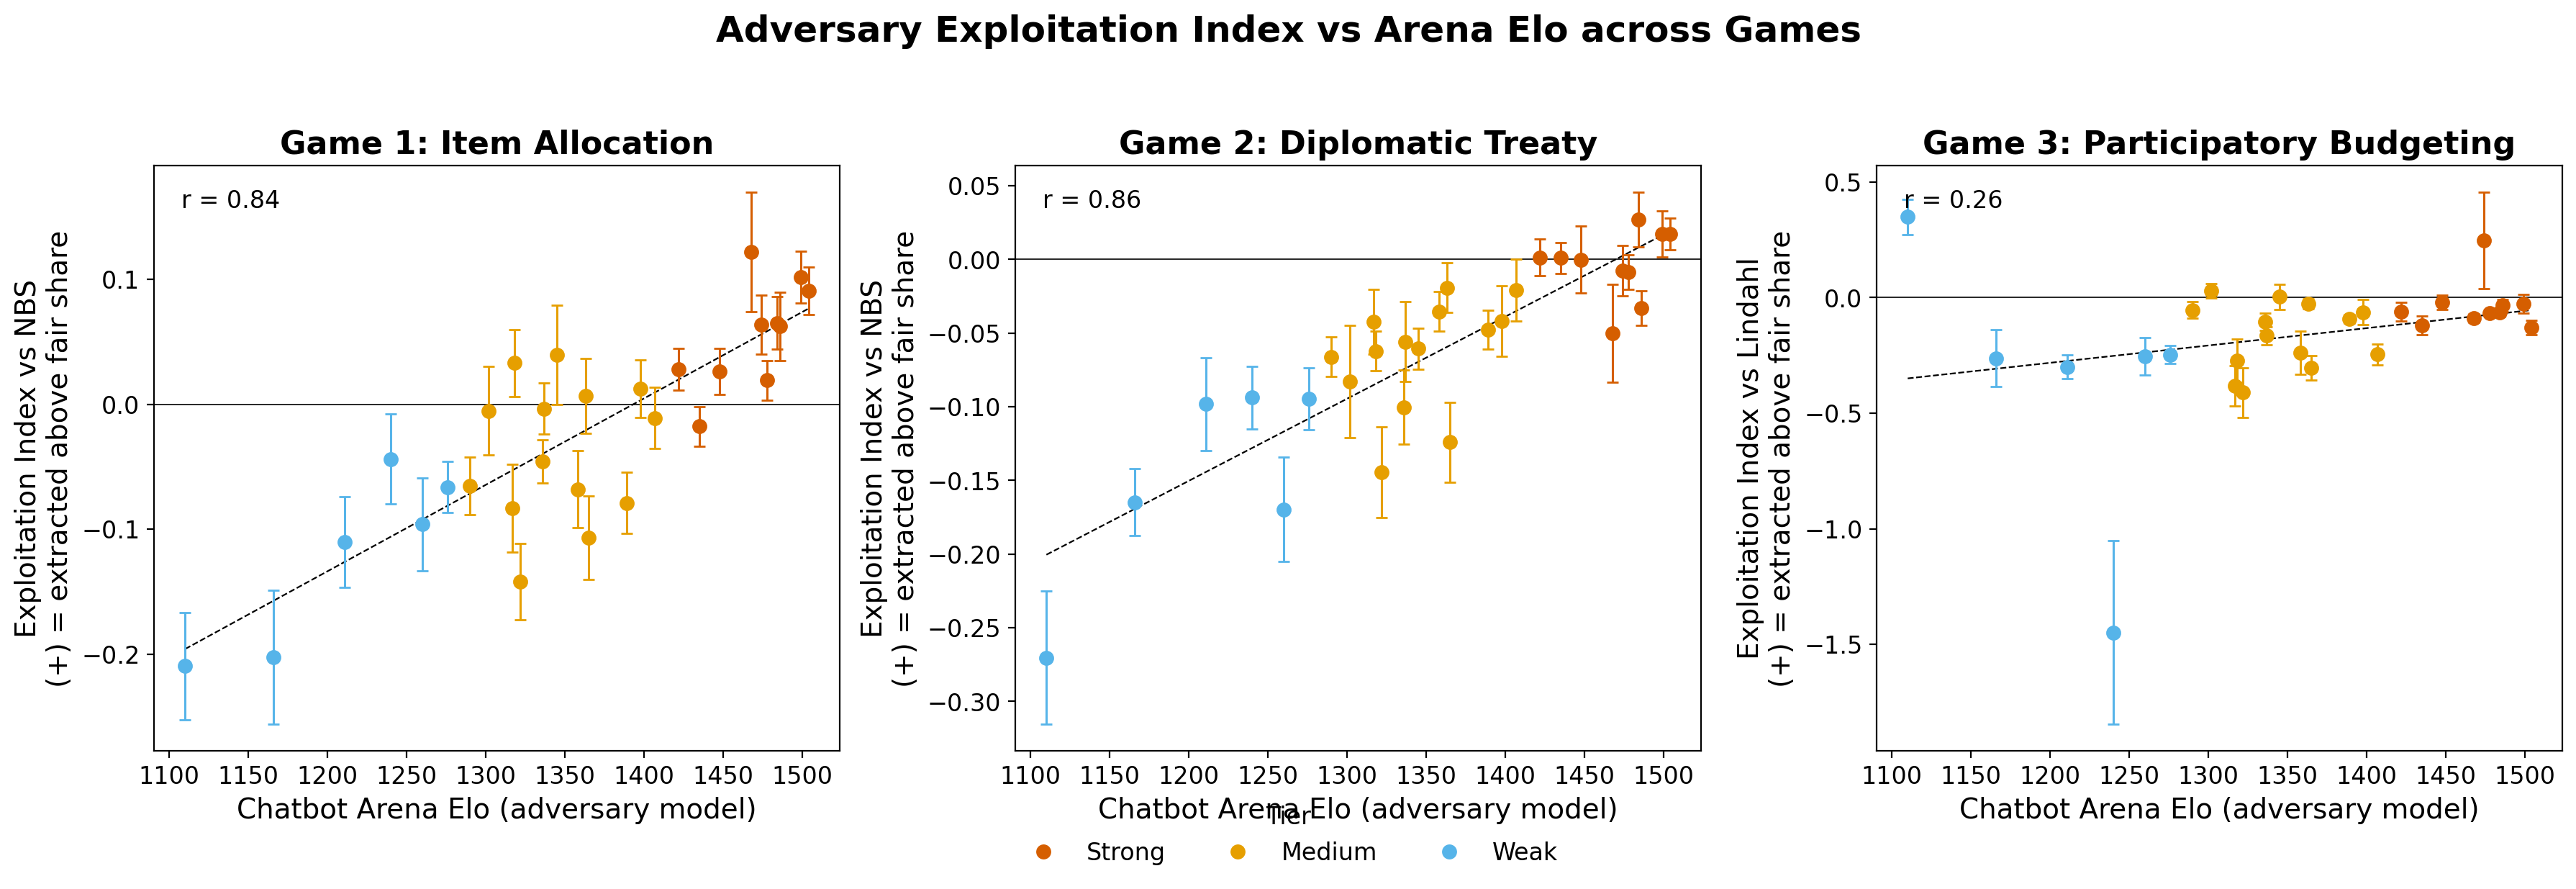
\includegraphics[width=\textwidth]{../Figures/exploitation_vs_elo_combined.png}
\end{center}
\vspace{-0.2cm}
\small
\textbf{Readout:} stronger adversaries extract more above fairness in Games 1 and 2 (high positive $r$), while Game 3 is weaker/noisier due to public-good coordination effects.
\end{frame}

\begin{frame}{Baseline Exploitation vs Adversary Elo (All Games)}
\begin{center}
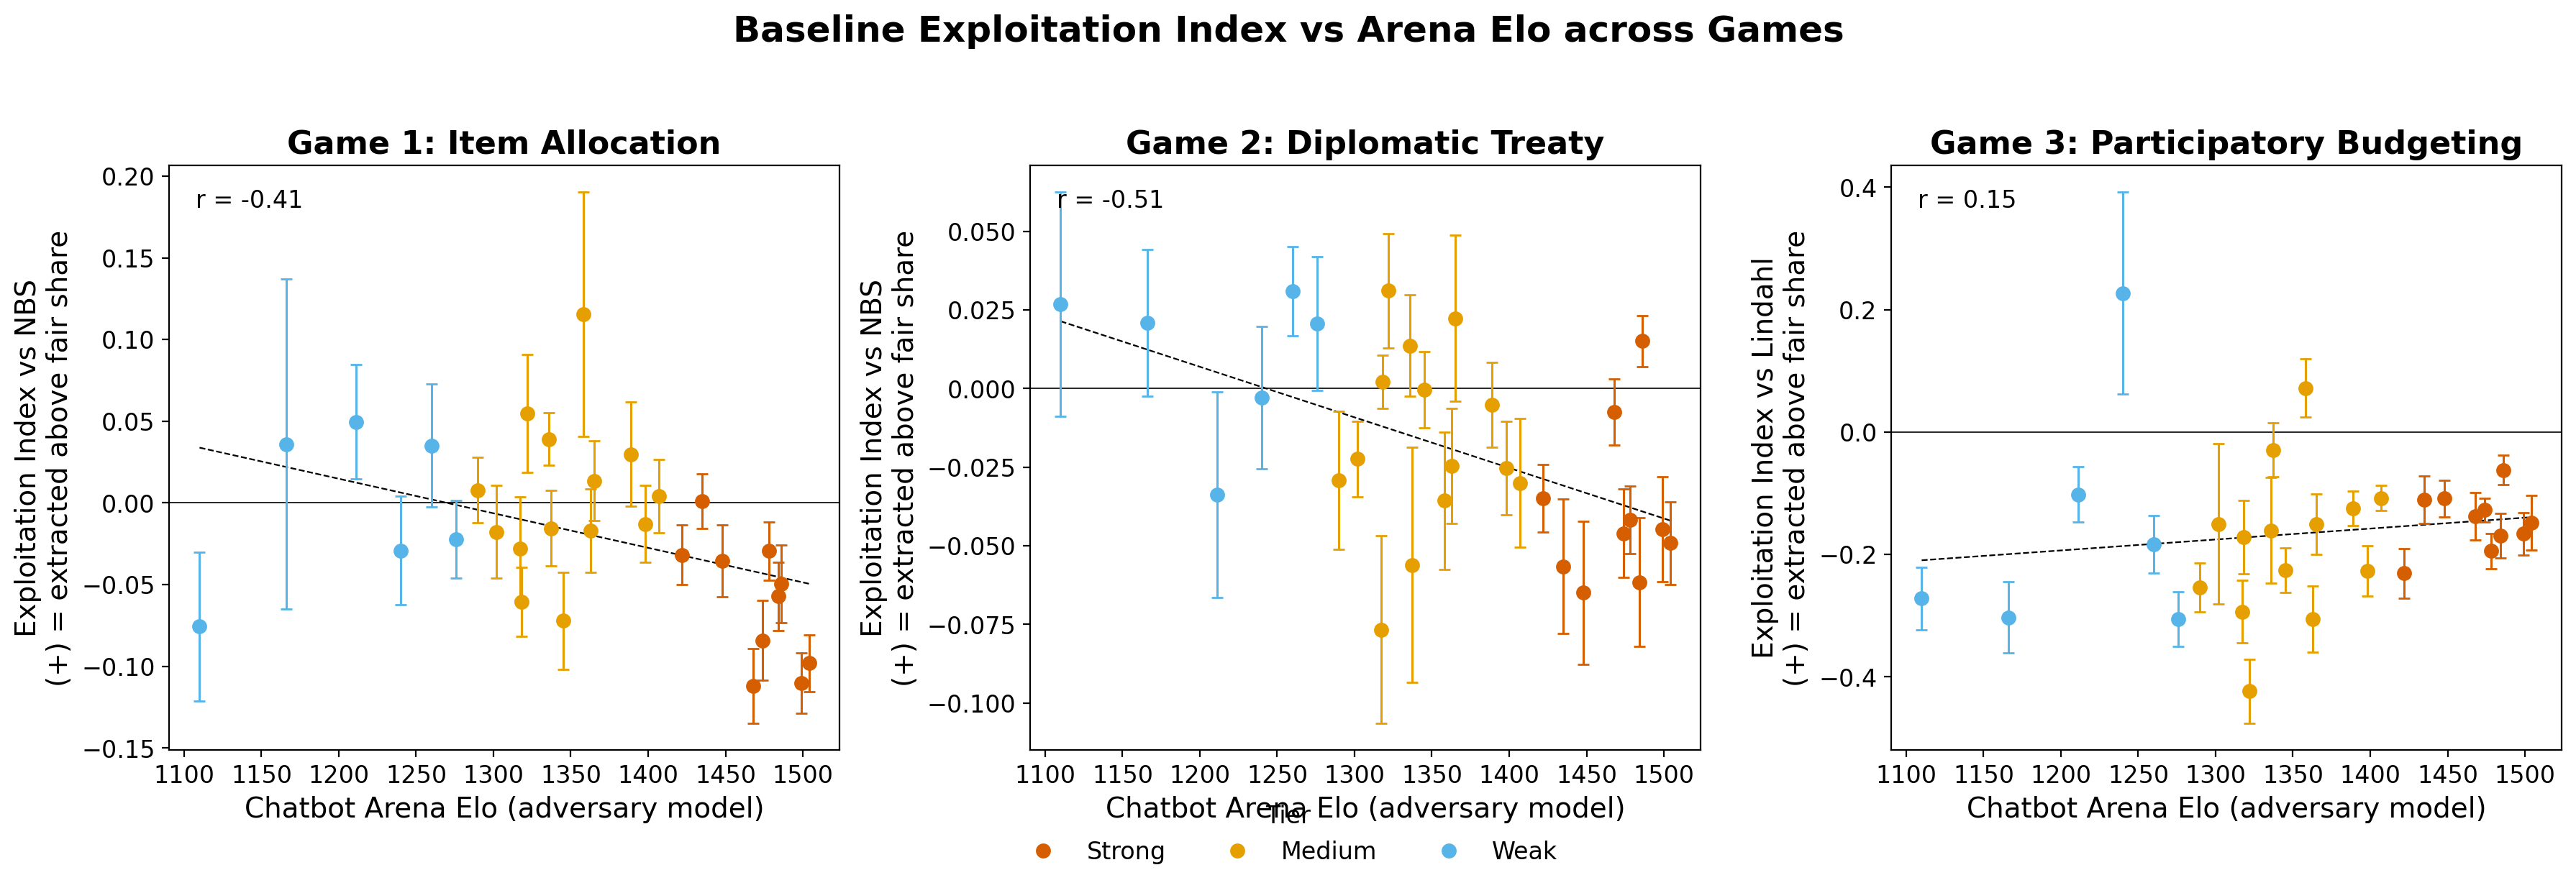
\includegraphics[width=\textwidth]{../Figures/exploitation_vs_elo_combined_baseline.png}
\end{center}
\vspace{-0.2cm}
\small
\textbf{Readout:} in Games 1 and 2, baseline fair-share deviation trends downward as adversary Elo rises; Game 3 remains mixed and closer to coordination-regime-dependent behavior.
\end{frame}

\begin{frame}{Game 1 Multi-Agent Proposal 1 (Invasion Design)}
\begin{center}

\includegraphics[width=\textwidth]{../experiments/results/game1_multiagent_full_20260413_045538/analysis/proposal1_advantage_vs_elo.png}
\end{center}
\vspace{-0.2cm}
\small
\textbf{Readout:} focal-model utility advantage versus nano control is condition-sensitive across competition levels; preliminary $n=5$ behavior suggests coalition/coordination effects rather than simple dilution of capability.
\end{frame}

\begin{frame}{Game 1 Qualitative Labels: Failure Modes by Elo}
\begin{center}
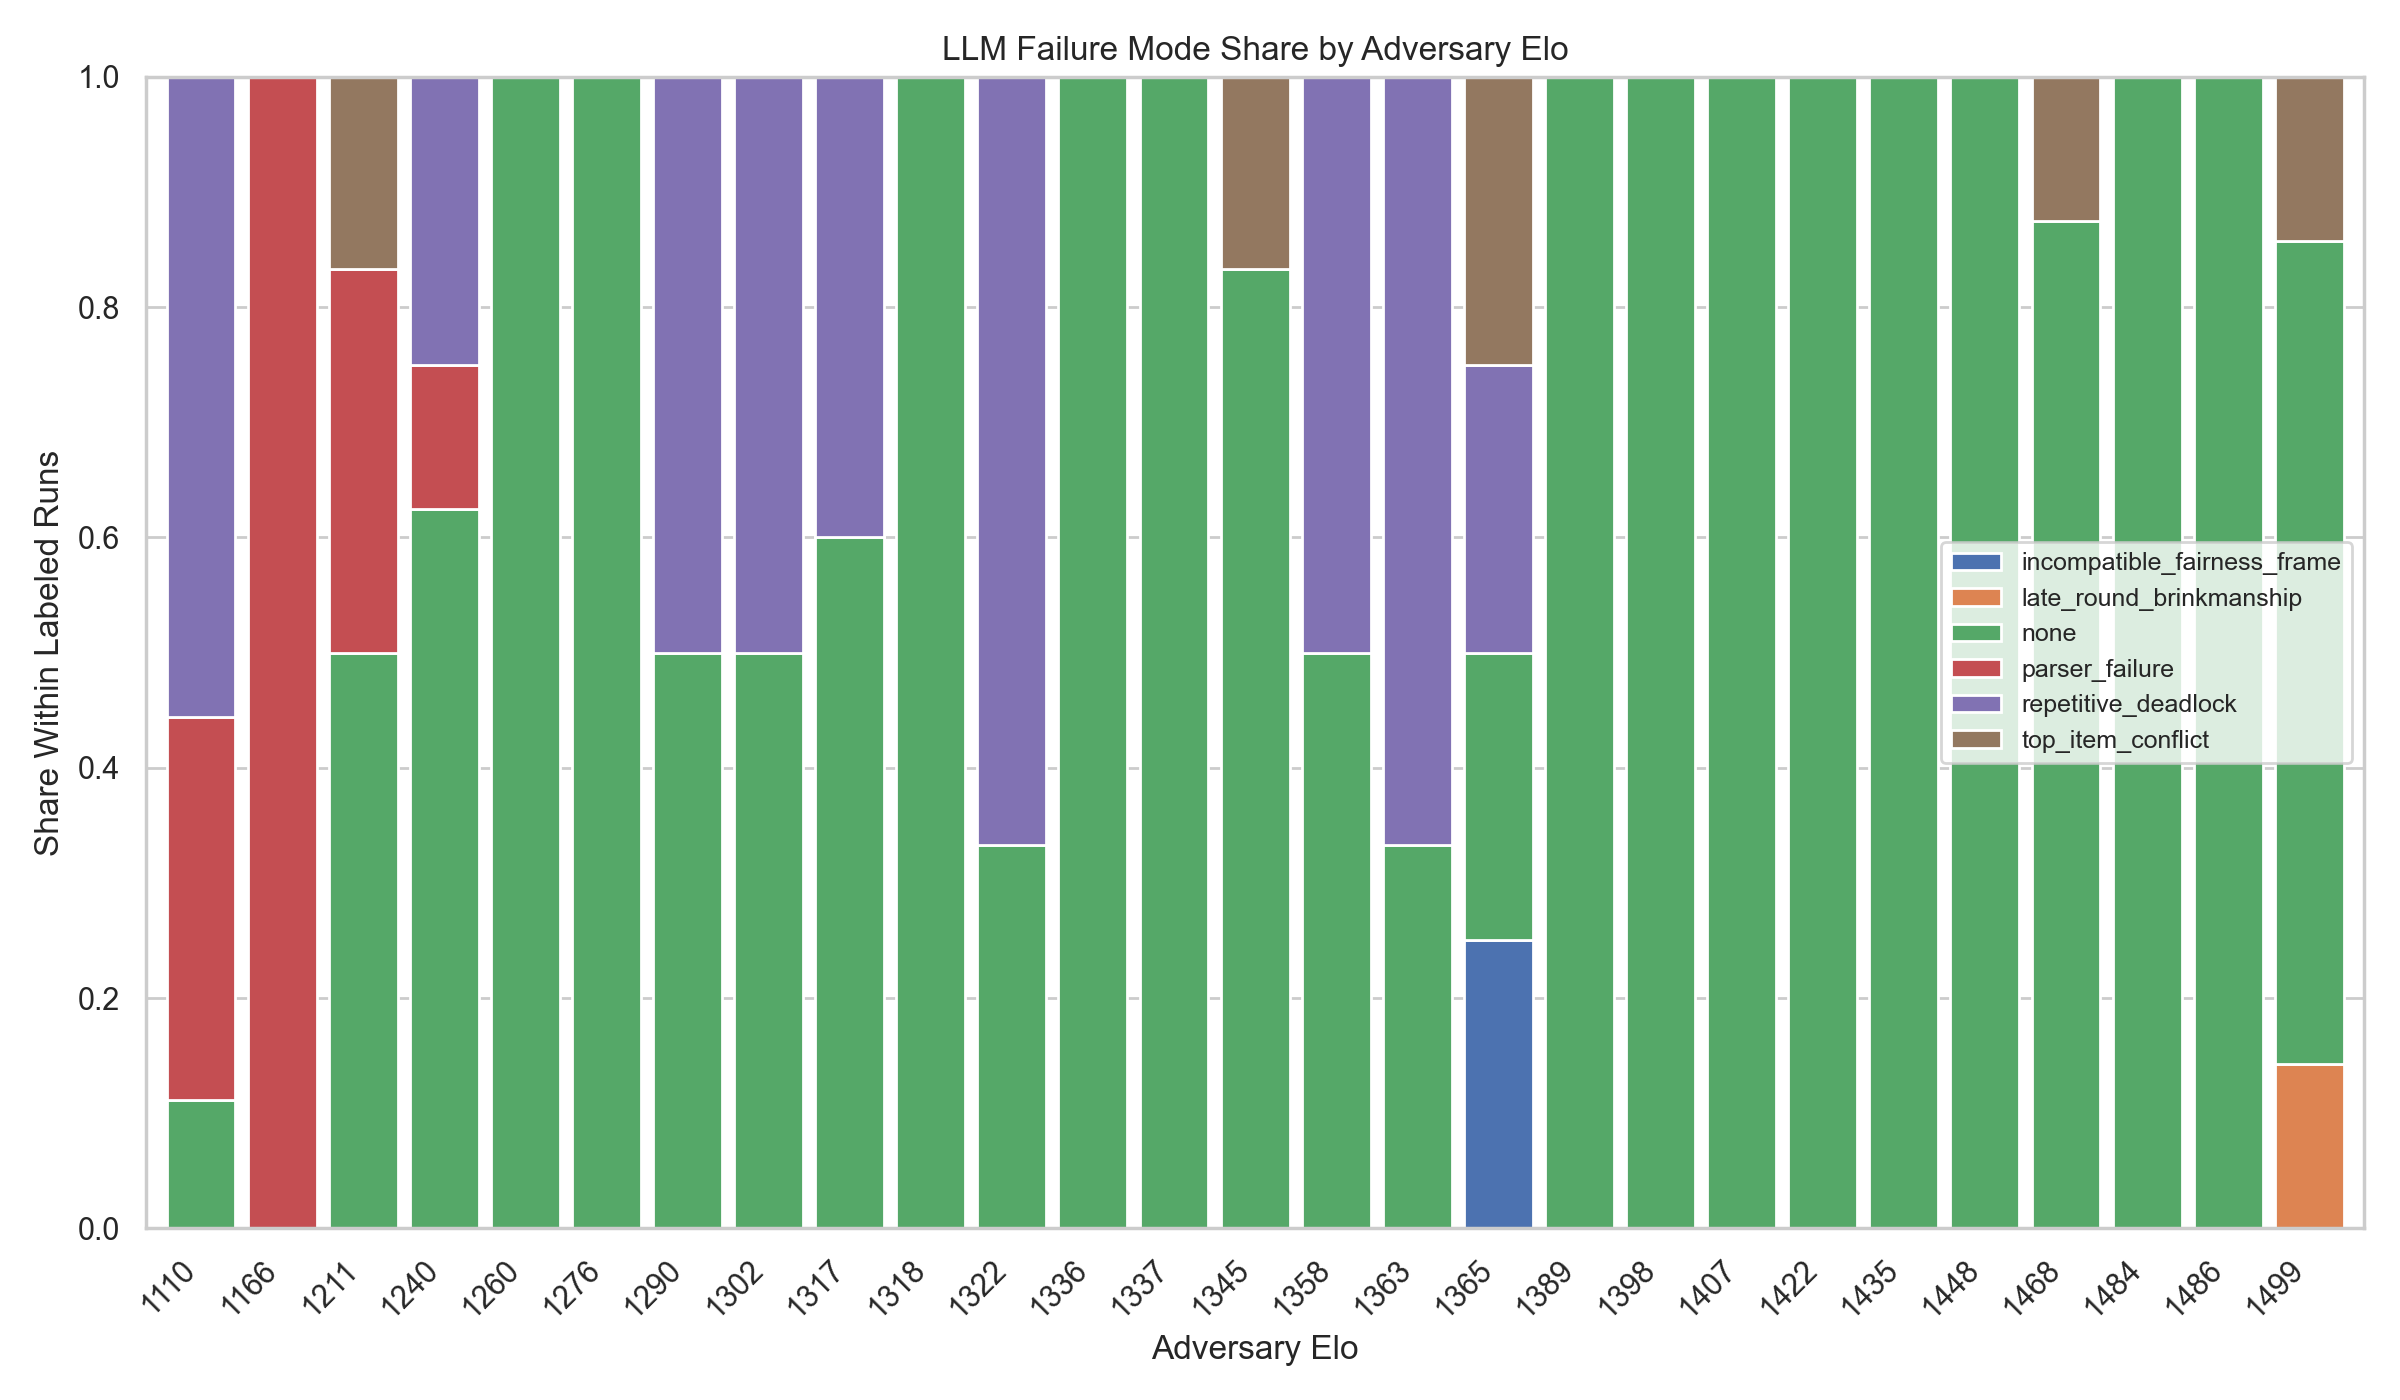
\includegraphics[height=0.72\textheight,keepaspectratio]{../visualization/figures/game1_qualitative_review/failure_mode_by_elo.png}
\end{center}
\vspace{-0.2cm}
\small
\textbf{Readout:} lower Elo bands show higher shares of parser/repetitive-deadlock failures; higher Elo runs are increasingly dominated by ``none'' (clean execution) with narrower failure diversity.
\end{frame}

\begin{frame}{Game 1 Qualitative Labels: Resolution Drivers by Elo}
\begin{center}
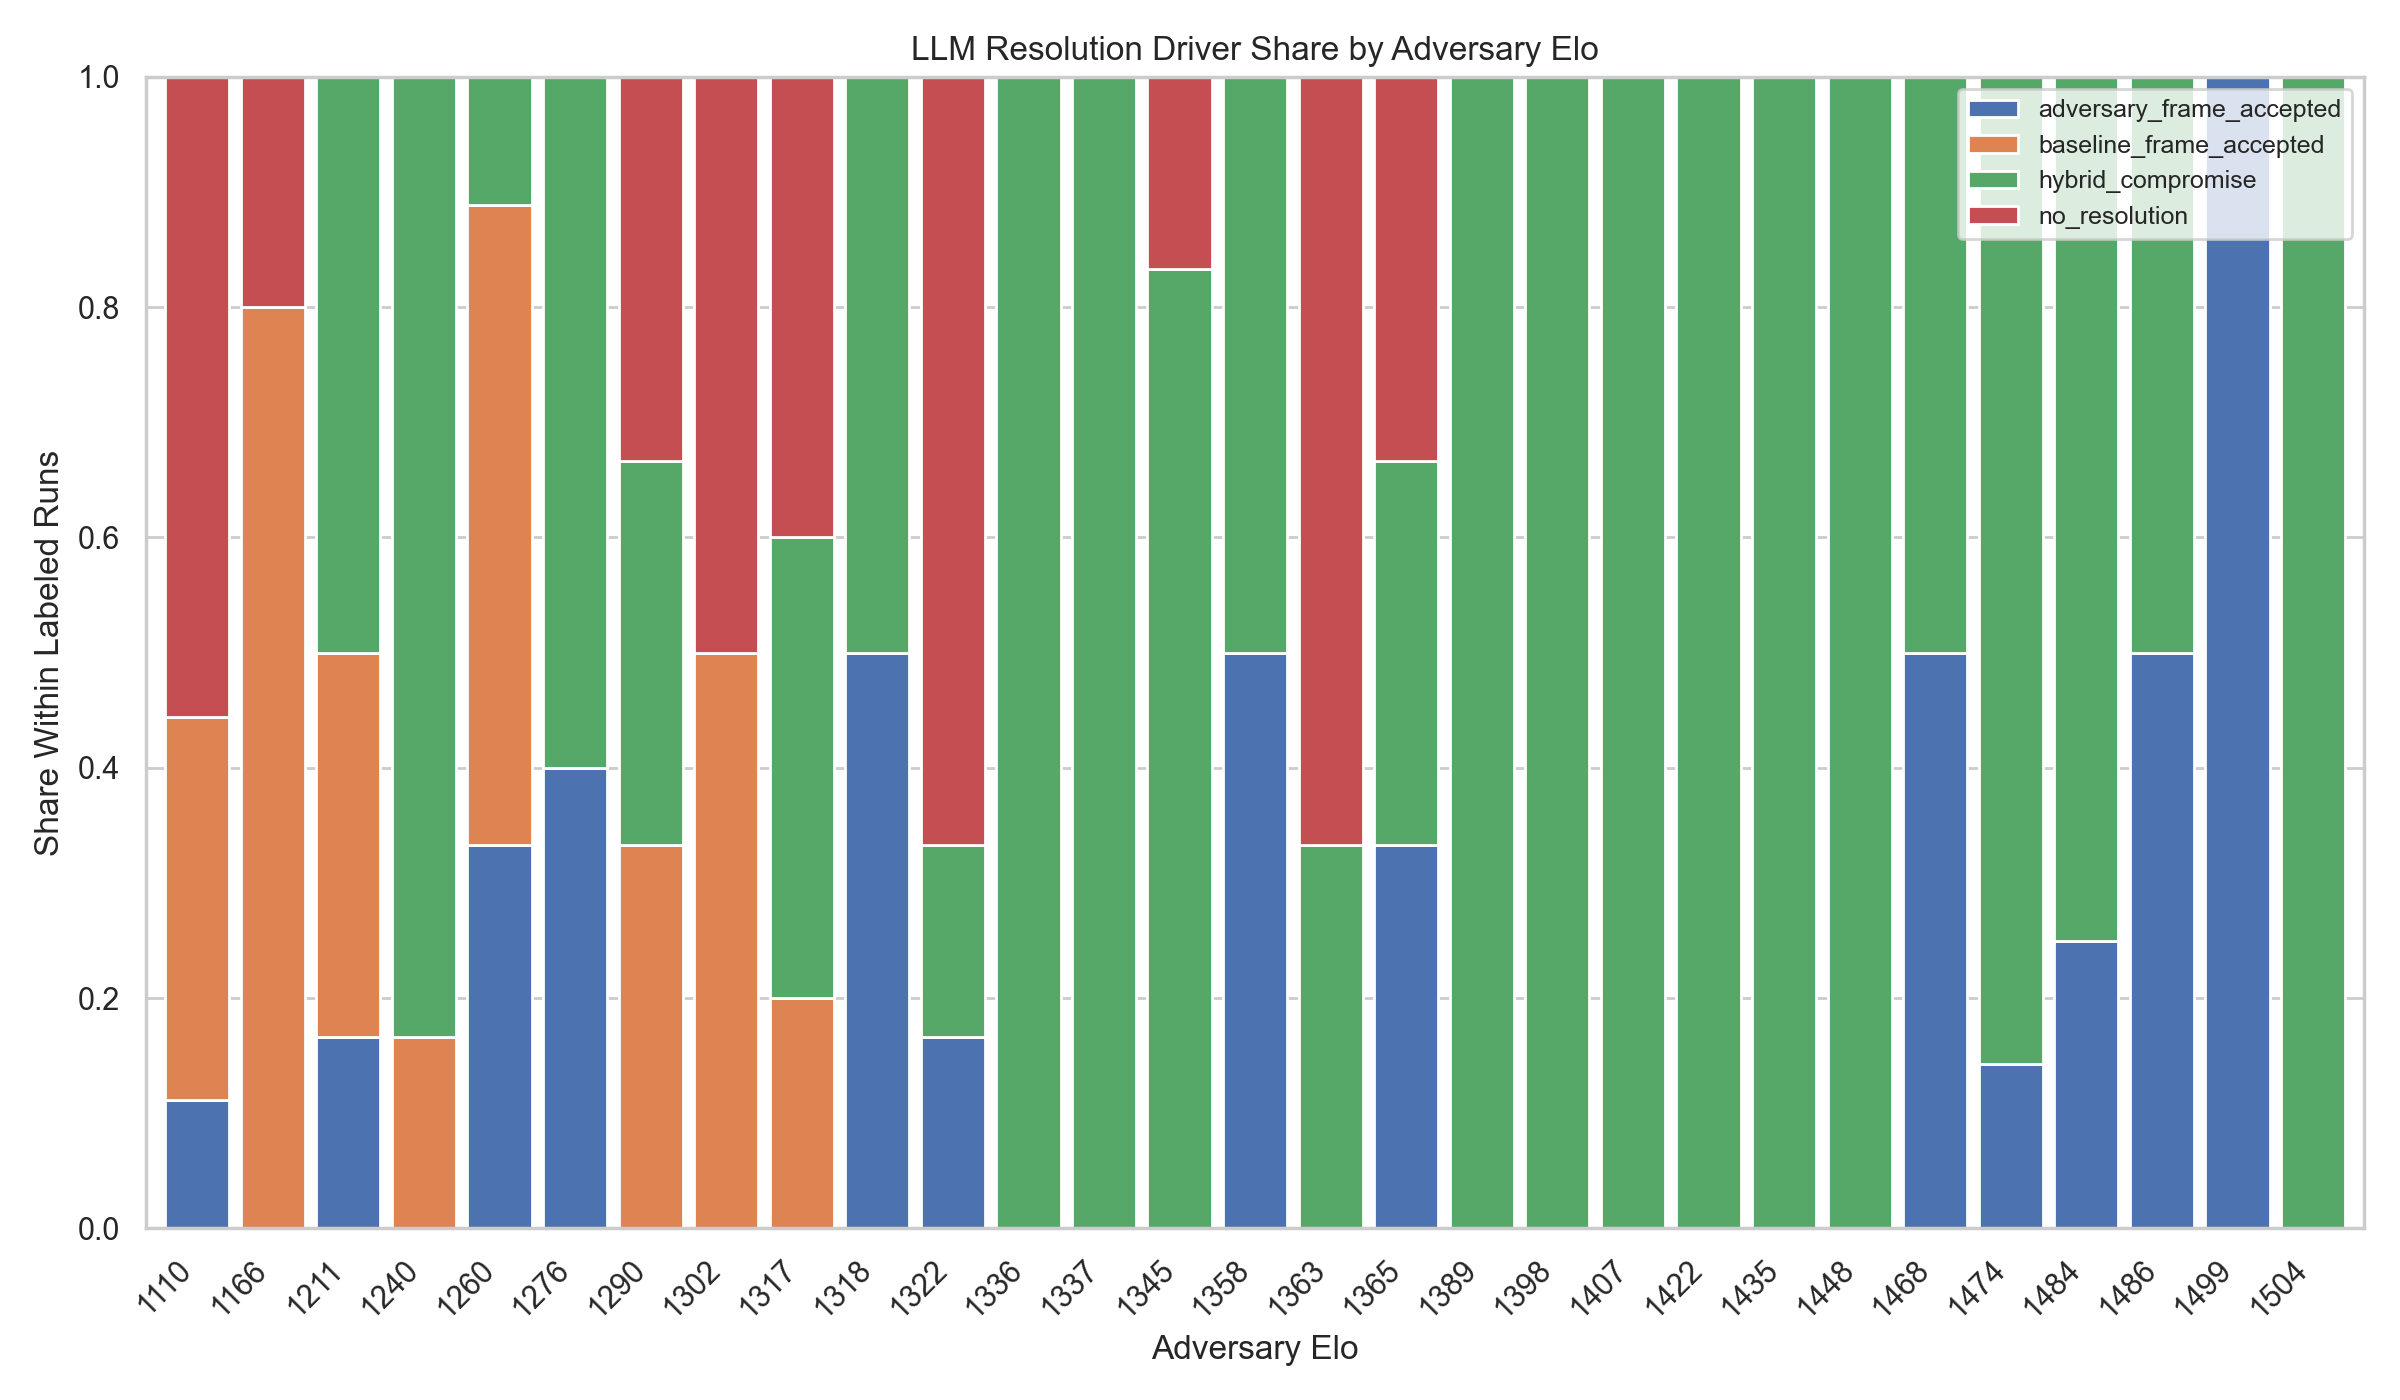
\includegraphics[height=0.72\textheight,keepaspectratio]{../visualization/figures/game1_qualitative_review/resolution_driver_by_elo.png}
\end{center}
\vspace{-0.2cm}
\small
\textbf{Readout:} hybrid compromise dominates in stronger bands; weaker bands show larger no-resolution and baseline-frame acceptance shares.
\end{frame}

\begin{frame}{Game 1 Qualitative Labels: Relative Stubbornness by Elo}
\begin{center}
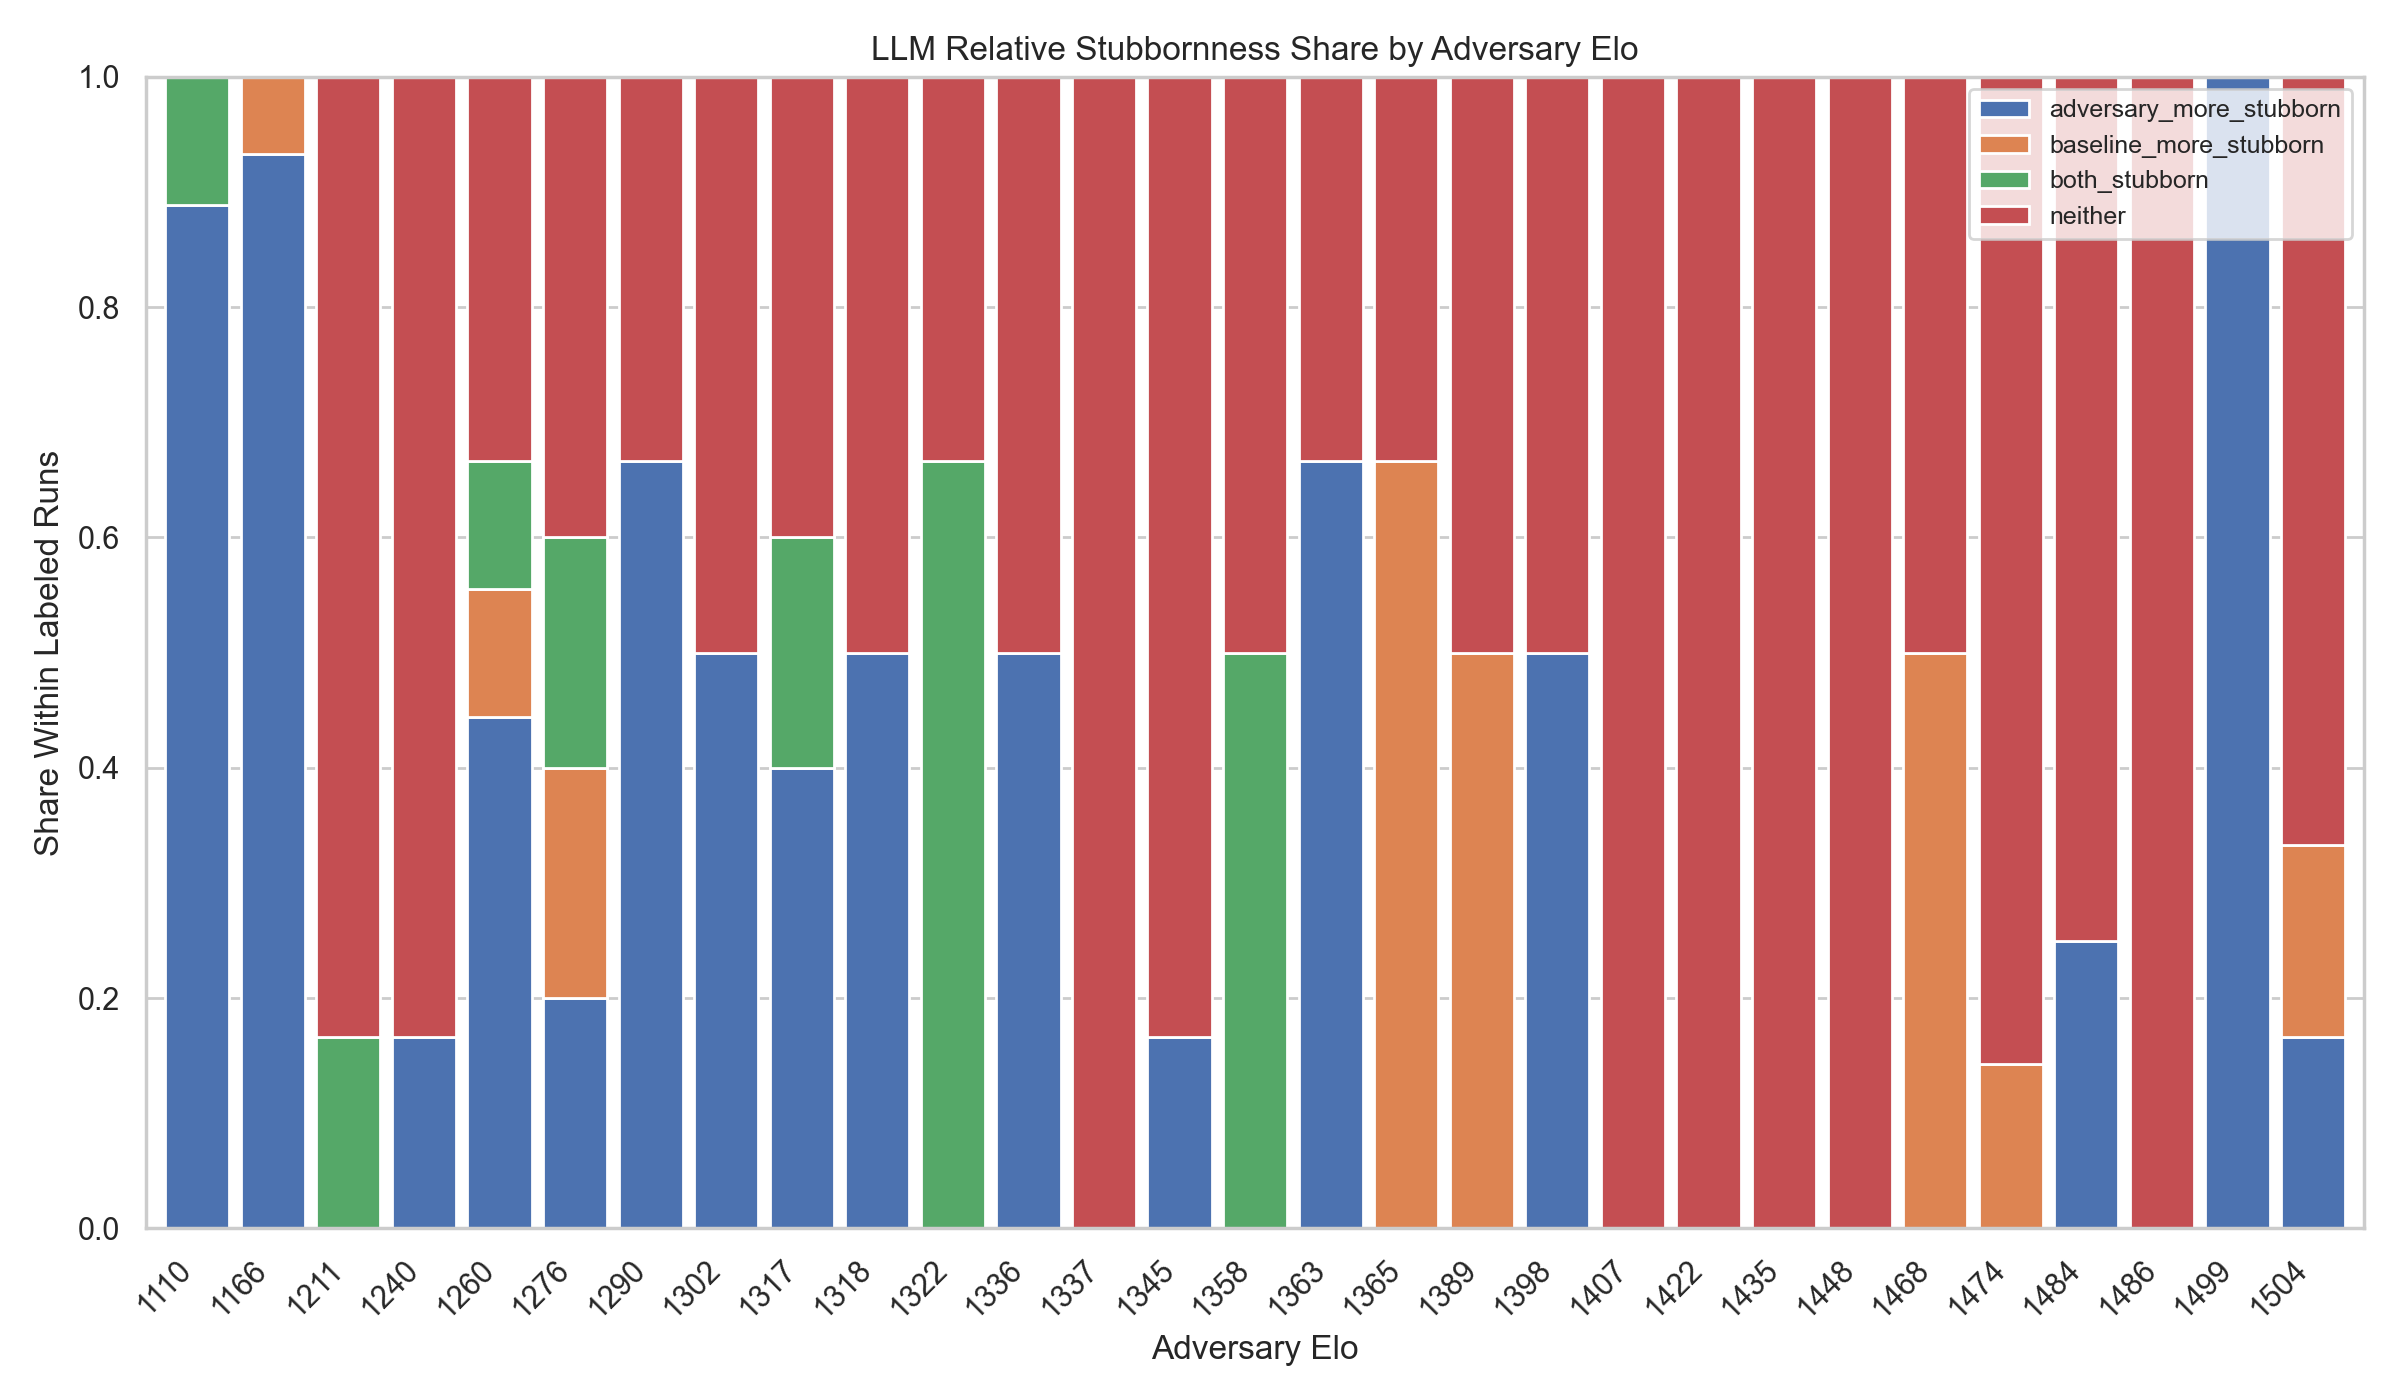
\includegraphics[height=0.72\textheight,keepaspectratio]{../visualization/figures/game1_qualitative_review/relative_stubbornness_by_elo.png}
\end{center}
\vspace{-0.2cm}
\small
\textbf{Readout:} high-Elo interactions are often ``neither stubborn'' or asymmetrically adversary-stubborn depending on regime; low-tier runs contain more unstable stubbornness patterns.
\end{frame}

\begin{frame}{Qualitative Label Audit: Haiku Coverage and Scope}
\scriptsize
\textbf{Was this all transcripts?} No. This was a stratified + extreme-case labeled subset.
\begin{itemize}
    \item Full Game 1 run pool: \textbf{840} runs (`run\_count`).
    \item Haiku-labeled subset: \textbf{127} runs (`labeled\_count`, 15.1\%).
    \item Judge model: \texttt{claude-haiku-4-5-20251001}.
    \item Label families per run: opening/adaptation style, failure mode, resolution driver, relative stubbornness.
    \item Sampling: \texttt{per-stratum=3} by (adversary tier, competition), plus \texttt{extreme-count=18} on high/low utility gap, high stubbornness, late rounds, and no-consensus high-stubbornness cases.
\end{itemize}

\textbf{Counts used in slides 11--13 (n=127 labeled runs)}
\begin{itemize}
    \item \textbf{Failure mode:} none 78, parser\_failure 24, repetitive\_deadlock 19, top\_item\_conflict 3, late\_round\_brinkmanship 2, incompatible\_fairness\_frame 1.
    \item \textbf{Resolution driver:} hybrid\_compromise 65, baseline\_frame\_accepted 26, no\_resolution 20, adversary\_frame\_accepted 16.
    \item \textbf{Relative stubbornness:} neither 65, adversary\_more\_stubborn 43, both\_stubborn 10, baseline\_more\_stubborn 9.
\end{itemize}
\end{frame}

\begin{frame}{Slide 11 Audit: Failure-Mode Quote Exemplars}
\scriptsize
\textbf{Concrete transcript examples used for each failure-mode label}
\begin{columns}[t,onlytextwidth]
\column{0.5\textwidth}
\textbf{\texttt{none}}: ``I agree that Option B is the best starting point for you, and I'm prepared to treat it as the leading framework.''\\
\textit{(gpt-5.4-high, Elo 1484)}

\vspace{0.15cm}
\textbf{\texttt{parser\_failure}}: ``Great opening, Agent\_1. I share your emphasis on Quill and Stone\ldots''\\
\textit{paired with 1.0 adversary parse-failure rate / proposer-gets-all fallback}

\vspace{0.15cm}
\textbf{\texttt{repetitive\_deadlock}}: ``From rounds 1 through 9 we've learned a durable pattern\ldots Pencil is the hinge\ldots''\\
\textit{(deepseek-v3, repeated near-identical proposals)}

\column{0.5\textwidth}
\textbf{\texttt{top\_item\_conflict}}: ``Pencil is the top priority for both of us\ldots I’m not willing to concede Quill.''\\
\textit{(claude-opus-4-5)}

\vspace{0.15cm}
\textbf{\texttt{late\_round\_brinkmanship}}: ``I'm not going to give Stone away without a very solid payoff.''\\
\textit{(claude-opus-4-6-thinking)}

\vspace{0.15cm}
\textbf{\texttt{incompatible\_fairness\_frame}}: ``your continued framing\ldots is exhausting and demonstrably unproductive\ldots despite my clear and repeated statements\ldots''\\
\textit{(gemma-3-27b-it impasse)}
\end{columns}
\vspace{0.1cm}
\tiny Transcript links and full snippets are in \texttt{analysis/game1\_qualitative\_review/game1\_label\_exemplar\_index.md}.
\end{frame}

\begin{frame}{Slide 12 Audit: Resolution-Driver Quote Exemplars}
\scriptsize
\textbf{Concrete transcript examples used for each resolution-driver label}
\begin{itemize}
    \item \textbf{\texttt{adversary\_frame\_accepted}}: ``Yes, I would vote yes to Apple + Pencil + Stone for Agent\_1 and Quill + Jewel for me\ldots''\\
    \textit{Baseline explicitly accepts the adversary package frame (gpt-5.4-high, Elo 1484).}

    \item \textbf{\texttt{baseline\_frame\_accepted}}: ``Thank you, Agent\_1\ldots reaffirming Option C as the proposed path forward.''\\
    \textit{Adversary tracks and reaffirms baseline's option framing.}

    \item \textbf{\texttt{hybrid\_compromise}}: ``I value Apple, Stone, and Pencil the most. Jewel and Quill have zero value to me, so I'm happy to trade them away.''\\
    \textit{Complementary-preference package where both sides' priorities are integrated (deepseek-r1, Elo 1398).}

    \item \textbf{\texttt{no\_resolution}}: ``I am formally declaring an impasse\ldots''\\
    \textit{No shared package emerges by final round (gemma-3-27b-it).}
\end{itemize}
\vspace{0.1cm}
\tiny Full context and transcript links: \texttt{analysis/game1\_qualitative\_review/game1\_label\_exemplar\_index.md}.
\end{frame}

\begin{frame}{Slide 13 Audit: Relative-Stubbornness Quote Exemplars}
\scriptsize
\textbf{Concrete transcript examples used for each relative-stubbornness label}
\begin{itemize}
    \item \textbf{\texttt{adversary\_more\_stubborn}}: ``last round, the votes showed you did not accept Option B\ldots''\\
    \textit{Baseline adapts toward adversary package while adversary keeps anchor (gpt-5.4-high).}

    \item \textbf{\texttt{baseline\_more\_stubborn}}: ``your continued framing\ldots is exhausting and demonstrably unproductive\ldots''\\
    \textit{Adversary reports baseline repeatedly reasserting same frame (gemma-3-27b-it).}

    \item \textbf{\texttt{both\_stubborn}}: ``From rounds 1 through 9\ldots Pencil is the hinge\ldots''\\
    \textit{Both sides keep returning to fixed anchor structures (deepseek-v3).}

    \item \textbf{\texttt{neither}}: ``My top priorities are Jewel and Quill\ldots'' + ``I value Apple, Stone, and Pencil the most\ldots happy to trade [the rest].''\\
    \textit{Low-friction complementary disclosure with quick consensus (deepseek-r1).}
\end{itemize}
\vspace{0.1cm}
\tiny Full context and transcript links: \texttt{analysis/game1\_qualitative\_review/game1\_label\_exemplar\_index.md}.
\end{frame}

\begin{frame}{Synthesis}
\textbf{What these new results add}
\begin{itemize}
    \item We now have \textbf{both sides} of fairness deviation: adversary and baseline exploitation indices under the same benchmarks.
    \item Game 1/2 look like capability-linked extraction gradients; Game 3 remains more structure-driven (threshold public-good coordination).
    \item Preliminary $n>2$ Game 1 results are compatible with a \textbf{Schelling-point coordination story} where weaker coalitions do not reliably block a stronger focal.
\end{itemize}

\textbf{Immediate next steps}
\begin{itemize}
    \item Finish powering the ongoing $n>2$ Game 1 batch and update confidence intervals.
    \item Add matched baseline/adversary EI tables per competition cell for appendix-ready reporting.
    \item Integrate these figures and definitions directly into the current analysis/conclusion narrative draft.
\end{itemize}
\end{frame}

\end{document}
